%===============================================================================
%   CLASSE ET PACKAGES                                                         %
%========================                                                      %
%	\documentclass[12pt,oneside,french,a4paper]{article} % twoside             %
	\documentclass[conference]{IEEEtran}                                       %
%===============================================================================
%	\usepackage{amsfonts}		% Ens. Math. : $\mathbb{R}$ = ens. des réels   %
	\usepackage{amsmath}		% Mathématiques                                %
	\usepackage{amssymb}		% Symbols, grec ; O pour la complexité : $\mathcal{O}$
%	\usepackage{array}			% Tableaux                                     %
%	\usepackage[french]{babel}	% Français                                     %
	\usepackage[english]{babel}	% Anglais                                      %
	\usepackage{booktabs}		% Tableaux pro                                 %
	\usepackage{cite}			% Recommandé pour IEEEtran                     %
	\usepackage{color}			% Pour utiliser les couleurs                   %
%	\usepackage{eurosym}		% Symbole Euro (\euro)                         %
%	\usepackage{fancybox}		% Cadres                                       %
%	\usepackage{fancyhdr}		% En-têtes, pieds de page                      %
	\usepackage{float}			% Gestion des flottants ([H] <-> HERE.)        %
	\usepackage{flushend}		% Équilibre les colonnes (\raggedend désactive)%
%	\usepackage[left=2cm, top=2cm, right=2cm, bottom=2cm]{geometry}	% Dimensions
	\usepackage{graphicx}		% Inclusion graphiques                         %
%	\usepackage{listings}		% Listings de code                             %
%	\usepackage{multicol}		% Édition sur plusieurs colonnes               %
%	\usepackage{multirow}		% Cellules tableaux sur plusieurs lignes       %
%	\usepackage{numprint}		% Nombres avec espacements (\numprint{+-4,5e6,7})
%	\usepackage{pdfpages}		% Inclusion de PDF                             %
%	\usepackage{setspace}		% Gestion interlignes                          %
%	\usepackage[normalem]{ulem}	% \uline \uuline \uwave \sout \xout \(dash|dot)uline
	\usepackage{xcolor}			% Texte en couleur                             %
	\usepackage{xspace}			% Espaces après macros                         %
%	\usepackage{hyperref}		% Liens hypertextes                            %
%===============================================================================
	\begingroup\expandafter\expandafter\expandafter\endgroup                   %
	\expandafter\ifx\csname directlua\endcsname\relax	% compilé avec LuaTeX ?%
%		\usepackage{lmodern}		% Fontes                                   %
%		\usepackage{mathptmx}		% Fontes Adobe Times Roman                 %
%		\usepackage{mathrsfs}		% Fontes amstex                            %
		\usepackage[utf8]{inputenc}	% Encodage                                 %
		\usepackage[T1]{fontenc}	% Encodage : T1 = Norme Latex (mais != par défaut)
	\else                                                                      %
%		\usepackage{luatextra}				% Paquet pour LuaTeX               %
%		\defaultfontfeatures{Ligatures=TeX}	% Conserver les ligatures          %
%		\setmainfont{Linux Libertine O}
%		\setsansfont{Linux Biolinum O}
%		\setmonofont{}
	\fi                                                                        %
%===============================================================================
%   OPTIONS, COULEURS, MACROS                                                  %
%=============================                                                 %
%	\hypersetup{                                                               %
%		linktoc=all,                                                           %
%		breaklinks,                                                            %
%		colorlinks,                                                            %
%		linkcolor=black,                                                       %
%		citecolor=black,                                                       %
%		urlcolor=blue,                                                         %
%		baseurl       = http://,                                               %
%		pdfpagelayout = OneColumn, % pdfpagelayout=SinglePage                  %
%		pdfstartpage  = 1,                                                     %
%		pdfcreator    = {\LaTeX{}},                                            %
%		pdfproducer   = {\LaTeX{}},% Contient automatiquement le compilateur   %
%		bookmarksopen = true,                                                  %
%		bookmarksdepth= 2,% montrer les sections et sous-sections              %
%		pdfauthor     = {Quentin MONNET, Lynda MOKDAD, Jalel BEN-OTHMAN},
%		pdftitle      = {Energy-balancing method to detect denial of service attacks in wireless sensor networks},
%		pdfsubject    = {A new algorithm for control nodes selection submitted to ICC 2014},
%		pdfkeywords   = {Wireless sensor networks; Reliability, availability, and serviceability; Energy-aware systems; Simulation}
%	}                                                                          %
%===============================================================================
	\definecolor{vert}{rgb}{0.11,0.47,0.11}                                    %
	\newcommand\apriori{\textit{a~priori}\xspace}                              %
	\newcommand\aposteriori{\textit{a~posteriori}\xspace}                      %
	\newcommand\defacto{\textit{de~facto}\xspace}                              %
	\newcommand\eg{\textit{e.g.}\xspace}                                       %
	\newcommand\ie{\textit{i.e.}\xspace}                                       %
	\newcommand\via{\textit{via}\xspace}                                       %
	\newcommand\etc{\textit{et~cætera}\xspace}                                 %
	\newcommand\Wsns{Wireless sensor networks\xspace}                          %
	\newcommand\wsns{wireless sensor networks\xspace}                          %
	\newcommand\Wsn{Wireless sensor network\xspace}                            %
	\newcommand\wsn{wireless sensor network\xspace}                            %
	\newcommand\dos{denial of service\xspace}                                  %
	\newcommand\bs{base station\xspace}                                        %
	\newcommand\BS{BS\xspace}			                                       %
	\newcommand\ch{cluster head\xspace}                                        %
	\newcommand\chs{cluster heads\xspace}                                      %
	\newcommand\CH{CH\xspace}                                                  %
	\newcommand\CHs{CHs\xspace}                                                %
	\newcommand\leach{\textit{LEACH}\xspace}                                   %
	\newcommand\cn{\textit{cNode}\xspace}                                      %
	\newcommand\cns{\textit{cNodes}\xspace}                                    %
	\newcommand\vn{\textit{vNode}\xspace}                                      %
	\newcommand\vns{\textit{vNodes}\xspace}                                    %
	\newcommand\nsiii{\textsf{ns-3}\xspace}                                       %
	\newcommand\todo[1]{\textcolor{red}{\textbf{TO DO: }#1}}                   %
%===============================================================================
%   META                                                                       %
%==========                                                                    %
\title{Energy-balancing method to detect denial of service attacks in \wsns}
\author{
\IEEEauthorblockN{Quentin \textsc{Monnet}}
\IEEEauthorblockA{Lab. LACL, Université Paris-Est\\
LACL (EA 4219), UPEC\\
F-94010 Créteil, France\\
quentin.monnet@lacl.fr}
\and
\IEEEauthorblockN{Lynda \textsc{Mokdad}}
\IEEEauthorblockA{Lab. LACL, Université Paris-Est\\
LACL (EA 4219), UPEC\\
F-94010 Créteil, France\\
lynda.mokdad@u-pec.fr}
\and
\IEEEauthorblockN{Jalel \textsc{Ben-Othman}}
\IEEEauthorblockA{Lab. L2TI, Université Paris 13\\
L2TI (EA 3043), UP13\\
F-93430 Villetaneuse, France\\
jbo@univ-paris13.fr}
}
%===============================================================================
%===============================================================================
%   START
%===========
\begin{document}

\maketitle

\begin{abstract}
The use of sensor networks has increased rapidly over the last years.
Due to their low resources, sensors come along with new issues regarding network security and energy consumption.

Focusing on the network availability, previous studies proposed to protect the network against \dos attacks with the use of traffic monitoring agents on some nodes.
But if the control nodes go down or get compromised, they leave the network unprotected.
To better fight against attacks, we try to enhance this solution by introducing an energy-aware and secure method to select these monitoring nodes (called \cns) in a clustered \wsn.
Our election process is done in accordance to their remaining reserves: nodes with the higher residual energy are selected.
We discuss limitations of this deterministic process concerning security and cluster coverage, and suggest as a workaround to designate new control nodes (called \vns).
Those \vns are responsible for monitoring the \cns by periodically enquiring about their remaining energy and ensuring that they do not lie during the election process (in attempt to keep their \cn role).
Finally, we present some experimental results obtained with the \nsiii simulator in order to analyze the impact of our proposal on the energy repartition in the network.
\end{abstract}
\begin{IEEEkeywords}
Wireless sensor networks; Reliability, availability, and serviceability; Energy-aware systems; Simulation
\end{IEEEkeywords}


% vim: set spelllang=fr foldmethod=marker:
\section{Réseaux de capteurs sans fil et déni de service}

\lettrineh{L}{a lutte} contre les attaques de type «déni de service» dans les réseaux de capteurs sans fil est le fil directeur des travaux présentés dans cet ouvrage.\linebreak
Les réseaux de capteurs sont constitués de petits appareils ---~les capteurs~--- équipés d'un module de communication sans fil.
Dispersés dans l'environnement à étudier, ces capteurs sont chargés de réaliser des mesures physiques, de les convertir en un signal numérique, et de les rapatrier pour un traitement plus approfondi à une station de base, qui fait office d'interface entre le réseau et l'utilisateur.
Cette collecte d'information est soumises aux contraintes en ressources des capteurs, dont les capacités en calcul, en mémoire, et dont la réserve d'énergie disponible en batterie sont limitées.

Mais les protocoles déployés ont su être adaptés: les capteurs sont aujourd'hui utilisés dans une multitude d'applications dans des domaines aussi variés que l'environnement, la santé, l'urbanisme, les transports, la domotique, et bien sûr le domaine militaire.
Liés à la fois aux avancées technologiques et à l'émergence de nouveaux usages dans l'exploitation des données, les concepts de «transports intelligents», de «villes intelligentes» ou d'«Internet des objets» se développent peu à peu et semblent promettre un usage de plus en plus intensif des réseaux de capteurs sans fil.

Toutefois, ces réseaux particuliers introduisent leur lot de problématiques: à côté des contraintes fortes en ressources se pose la question de la sécurité, dont la mise en place est une nécessité absolue pour les applications médicales ou militaires par exemple.
Alors que les mécanismes d'authentification et de chiffrement font appel, dans la plupart des systèmes informatiques, à des protocoles cryptographiques couteux en ressources, il a fallu adapter les mécanismes au monde des capteurs.
Mais la sécurité comporte d'autres volets, et la disponibilité des réseaux, suivant le contexte, peut s'avérer tout aussi essentielle.

En résumé, le problème se pose ainsi: comment prévenir, ou à défaut comment détecter puis contourner, tout en économisant les ressources des capteurs, une action d'origine malveillante qui viserait à mettre le réseau hors service?
Cette thèse s'appuie sur l'attribution d'un rôle de surveillance à certains des capteurs, chargés de détecter des comportements hostiles au sein du réseau, et de prévenir leurs pairs lorsqu'une attaque est détectée.

C'est notamment le processus de sélection dynamique de ces capteurs de surveillance qui fait l'objet d'une étude poussée.
Plusieurs solutions sont proposées: une sélection aléatoire, permettant d'obtenir statistiquement une bonne couverture du réseau; une sélection basée sur l'énergie résiduelle des capteurs, dont l'avantage est d'offrir une meilleure répartition de la charge (en termes de consommation énergétique) dans le réseau; et enfin un processus d'élection démocratique, basé sur des scores de réputation, qui améliore encore la sécurité du dispositif.

Mais en sus des algorithmes concrets, il est parfois utile de pouvoir représenter un processus sous un aspect plus formel.
Validées par des simulations, certaines des méthodes proposées sont également modélisées à l'aide de chaines de \textsc{Markov} ou de réseaux de \textsc{Petri} particuliers.
En fin d'étude, les jeux quantitatifs sont utilisés pour caractériser à plus haut niveau le système comportant un capteur corrompu et des capteurs de surveillance.
\pagebreak %%%%%%%%%%%%%%%%%%%%%%%%%%%%%%%%%%%%%%%%%%%%%%%%%%%%%%%%%%%%%%%%%%%%

Le but des travaux présentés dans cette thèse est donc de proposer, dans un temps, un ensemble de méthodes de détection et de réaction efficace aux attaques de déni de service, tout en économisant ou en répartissant au mieux la consommation énergétique des capteurs pour prolonger le plus possible la durée de fonctionnement du réseau.
Les outils de modélisation fournis permettent à la fois de valider ces méthodes, de mieux les comprendre, et avec un peu de chance, de servir de base dans le futur pour la conception de mécanismes toujours plus performants.


% vim: set spelllang=fr foldmethod=marker:

\lettrineh{L}{e \chapref{sa}} expose un algorithme de sélection pseudo-aléatoire des nœuds de surveillance.
L'un des inconvénients de cet algorithme est que l'énergie résiduelle des capteurs, \cad le niveau d'énergie restant dans leur batterie, n'est pas mesurée, et surtout n'est pas prise en compte lors du processus de renouvellement des \cns.
Pourtant, la surveillance que ces derniers mènent dans leur cluster entraine une consommation énergétique accrue, puisqu'ils doivent demeurer en écoute sur le médium de façon continue.

Dans ce chapitre, une deuxième méthode de sélection des \cns est introduite.
Le concept initial de l'algorithme est extrêmement simple: à chaque renouvellement du processus, l'énergie résiduelle des capteurs est évaluée, et ceux possédant le plus de réserves deviennent \cns.
Le but de cette méthode est évidemment d'atteindre une meilleure répartition de la consommation d'énergie dans le cluster: les capteurs possédant le plus haut niveau de charge de leur batterie se verront attribuer le rôle qui consomme le plus d'énergie.

Néanmoins, la perte de l'aspect aléatoire au profit d'une méthode purement déterministe va entrainer un certain nombre de contraintes en termes de sécurité et de couverture spatiale.
Il faut donc mettre en place des parades face aux nœuds compromis qui tenteraient de conserver \textit{ad~vitam~æternam} le rôle de \cn en falsifiant leur niveau d'énergie.
Un nouveau type de nœuds, les \vns, viennent ici prévenir les tentatives de fraudes, tandis que le \ch veille à la couverture correcte du réseau par les \cns.
Les performances obtenues à l'aide de ce second mécanisme de sélection sont elles aussi étudiées à travers un jeu de simulations.

\section{Mécanisme de sélection des \cns}\label{se:sec:proposal}

    \subsection{Utilisation des \vns pour sécuriser le processus de sélection}\label{se:subsubsec:elec1}

Les hypothèses présentées en début de \chapref{sa} (\ssref{sa:ssec:hypotheses}) demeurent valables ici.
Le processus de sélection dans ce chapitre repose sur l'énergie restante pour chaque nœud au moment du renouvellement.
Cette énergie disponible dans la batterie est dite «énergie résiduelle».
Afin de répartir au mieux la charge, les nœud possédant le plus d'énergie en réserve sont sélectionnés pour assurer la tâche qui consomme le plus.
Mais l'usage de la valeur d'énergie résiduelle comme critère de sélection présente un inconvénient notable: il n'y a aucun agent, dans le réseau, capable de mesurer de façon fiable le niveau d'énergie présent dans la batterie d'un nœud donné, si ce n'est ce nœud lui-même.
Les nœuds voisins d'un nœud $N$ peuvent tout au plus enregistrer les messages envoyés par $N$, et en inférer une valeur approximative de l'énergie consommée.
Mais ils ne connaissent ni le niveau d'énergie initial de $N$ (au moment du déploiement du réseau) ni l'énergie dépensée par $N$ lors de l'écoute du médium de transmission, la consommation approximative calculée ne permet pas de déduire le niveau d'énergie résiduelle avec une précision suffisante pour classer les nœuds de façon fiable sur ce critère.

Aussi la seule façon d'obtenir le niveau de charge de la batterie d'un nœud est-elle de le lui demander.
L'algorithme de sélection proposé s'écrit donc de la manière suivante:
\begin{enumerate}
    \item Au cours d'une première phase, chaque nœud évalue la valeur de son énergie résiduelle et la transmet au \ch;
    \item Une fois cette phase terminée (lorsque le \ch a reçu la valeur de chaque nœud, ou lorsque le délai d'attente a expiré), le \CH sélectionne les $n$ capteurs possédant le niveau d'énergie le plus élevé (où $n$ représente le nombre de \cns que l'on souhaite obtenir durant chaque cycle) et envoie à ceux-ci un message de notification pour leur assigner leur rôle de \cn.
\end{enumerate}
Cet algorithme est déterministe, et élimine tout aspect aléatoire du processus de sélection.
La règle est simple: les $n$ nœuds possédant le plus d'énergie en réserve au moment de la sélection sont désignés.
Comme le rôle de \cn est censé impliquer une consommation plus élevée en ressources énergétiques, la rotation des rôles est théoriquement assurée.

Mais l'aspect entièrement déterministe du processus peut aussi représenter une faille qui pourrait être exploitée par des nœuds compromis souhaitant s'assurer d'être sélectionnés.
Un attaquant a effectivement intérêt à faire attribuer le rôle de \cn aux nœuds qu'il a compromis, car cela lui permet:
\begin{itemize}
    \item de réduire le nombre de \cns légitimes dans le réseau capables de détecter les capteurs compromis;
    \item de signaler au \ch des capteurs «innocents» comme étant compromis, dans le but de les faire exclure du réseau.
\end{itemize}
Quand un algorithme de sélection (pseudo-)aléatoire est appliqué, un nœud compromis peut très bien être désigné pour un cycle, mais il perdra rapidement son rôle de surveillance, pour les cycles suivants.
Même avec un processus d'auto-désignation (basé sur le modèle de \leach par exemple), les nœuds compromis pourraient tenter de conserver leur rôle de \cn sur plusieurs cycles, mais cela n'empêcherait pas des capteurs légitimes de s'auto-désigner également.
Avec un processus déterministe, les nœuds compromis peuvent en revanche monopoliser la plupart des rôles de \cns.
Tout ce qu'ils ont à faire, pour en arriver là, consiste à annoncer un niveau de charge batterie plus élevé que celui des capteurs légitimes lors de la première phase de l'algorithme de sélection.
Ils sont alors assurés d'être désignés \cns; et s'il se trouve y avoir au moins $n$ nœuds compromis au sein du cluster, ils peuvent de cette manière accaparer les $n$ rôles de \cn et désactiver du même coup le mécanisme de détection dans son intégralité.
L'attaque devient alors impossible à détecter et à contrer.

Pour empêcher les capteurs de «mentir» lorsqu'ils annoncent leur valeur d'énergie résiduelle, l'assignation d'un nouveau rôle à certains des voisins de chaque \cn est proposée.
Ces nœuds, que nous appelleront désormais \vns (comme pour \textit{nœuds de vérification}), seront responsables de vérifier la consommation en énergie des nœuds de surveillance.
Une fois que la sélection des \cns est réalisée, chaque voisin d'un \cn nouvellement désigné choisit à partir d'un seuil de probabilité prédéfini s'il sera ou non \vn pour ce \cn.
Un capteur peut assumer le rôle de \vn pour plusieurs \cn différents, du moment qu'il s'agit de nœuds voisins.

Si le rôle de \vn s'avère trop gourmand en énergie, il devient inutile: autant déployer dès le départ, dans ce cas, un mécanisme de sélection pseudo-aléatoire des \cns.
Aussi les \vns ne doivent-ils pas demeurer en permanence à l'écoute du médium, comme le font les \cns.
Ils se contentent d'envoyer, de temps en temps, une requête au \cn qu'ils surveillent, pour lui demander son niveau d'énergie.
Ils conservent la réponse du \cn en mémoire.

Une fois qu'ils ont collecté suffisamment de données, les \vns essayent d'établir une corrélation entre le modèle théorique de la consommation du \cn surveillé, et les valeurs que celui-ci annonce (valeurs obtenues à la fois lors des phases de sélection et en réponse aux requêtes).
Quatre cas sont alors susceptibles de se produire:
\begin{enumerate}
    \item La consommation en énergie annoncée par le \cn ne correspond pas du tout au modèle théorique: il y a alors une forte probabilité pour que le nœud soit corrompu, et cherche à accaparer le rôle de \cn. Il est dénoncé au \ch;
    \item La consommation annoncée correspond très exactement au modèle théorique: le capteur est probablement un nœud compromis qui tente d'être sélectionné tout en échappant à la détection des \vns. Autrement dit: le nœud est compromis, mais il adapte son comportement par rapport au point précédent. Mais il est quasiment impossible en pratique que les valeurs théoriques et empiriques soient exactement identiques, sans la moindre marge d'erreur. Le capteur est donc dénoncé au \ch;
    \item La consommation correspond à peu près aux valeurs du modèle théorique, mais elle n'évolue pas dans le sens de la consommation réelle observée localement par les \vns (l'évolution locale dans le temps du \cn devrait être grossièrement similaire à celle des \vns, puisqu'ils sont voisins, mais ce n'est pas le cas). Il s'agit probablement d'un nœud compromis qui adapte son comportement par rapport aux deux premiers points, par exemple en décrémentant son énergie des montants minimum imposés par la marge d'erreur définie vis à vis du modèle théorique. Le nœud est dénoncé au \ch;
    \item La consommation annoncée correspond grossièrement au modèle théorique, et évolue dans le sens de la consommation locale observée par les \vns. Que le nœud soit compromis ou non, il adopte ici un comportement normal, et est autorisé à endosser le rôle de \cn.
\end{enumerate}
Si un \vn est compromis, il peut tenter de faire exclure le \cn légitime qu'il observe.
Le \ch doit donc recevoir les rapports de plusieurs \vns distincts (selon un seuil prédéterminé) avant de considérer un \cn comme étant réellement compromis.
Dans une certaine mesure, cette précaution permet aussi de protéger un \cn légitime des erreurs (faux positifs) de ses \vns.

Le recours au rôle de \vn assure ainsi que seuls les nœuds annonçant un niveau d'énergie résiduelle plausible seront autorisés à agir en temps que \cns.
Comme ce dernier rôle consomme plus d'énergie que le relevé et la transmission des mesures sur l'environnement des capteurs, les nœuds sélectionnés pour être \cns verront tôt ou tard leur énergie résiduelle descendre sous le niveau des nœuds assurant leurs fonctions de base; une fois ce stade atteint, ils sont assurés de perdre leur rôle pour le cycle suivant.
On remarquera que les points~2 et~3 énoncés ci-dessus correspondent à un nœud compromis qui décrémente volontairement son énergie annoncée au cours du temps; même si des irrégularités peuvent être détectées et le nœud compromis être ainsi démasqué, le seul fait qu'il applique ce comportement assure tout de même que le capteur compromis cessera d'être désigné \cn pour un cycle ou pour un autre dans le futur.

Le modèle énergétique implémenté par les \vns pour vérifier les affirmations des \cns ne doit pas être trop lourd, mais il doit demeurer suffisamment précis pour pouvoir déterminer si un \cn s'en éloigne véritablement, tout en limitant les faux positifs.
Nous proposons ici d'utiliser le modèle de diffusion de \textsc{Rakhmatov} et \textsc{Vrudhula}~\cite{RV01}.\label{se:rakvru-formula}
Ce choix repose sur plusieurs observations:
\begin{itemize}
    \item Ce modèle fournit une approximation assez précise de la consommation réelle d'une batterie, et tient compte des processus chimiques internes à la batterie tels que les effets de récupération (\textit{recovery effect} en anglais) ou de perte de capacité selon la tension de décharge (\textit{rate capacity effect});
    \item Il s'agit de l'un des modèles implémentés dans \nsiii, ce qui permet, pour les simulations basées sur ce logiciel, de bénéficier d'une implémentation déjà existante, et surtout d'un modèle théorique parfait. Il ne faut pas craindre cependant que ce modèle ne soit «trop parfait» pour être utilisé par les \vns, étant donné que ces derniers estimeront l'énergie consommée par les \cns à partir de messages émis par ces derniers, sans connaissance des mécanismes internes au nœud (calcul, écoute) comme le fait le cœur du simulateur. Les valeurs calculées par les \vns demeurent donc approximatives par rapport à la consommation des \cns réellement calculée par \nsiii.
\end{itemize}
Le modèle de diffusion de \textsc{Rakhmatov} et \textsc{Vrudhula} se réfère aux réactions chimiques qui se produisent à l'intérieur de l'électrolyte de la batterie, et elle est résumée par l'\equaref{se:eqn:rvdm}
\begin{equation}
    \label{se:eqn:rvdm}
    \sigma(t) = \underbrace{\int_{0}^{t} i(\tau) \, \mathrm d\tau}_{l(t)} \;+\; \overbrace{\int_{0}^{t} i(\tau) \left(2 \sum_{m=1}^{\infty} \exp^{-\beta^2 m^2 (t-r)} \right) \mathrm d\tau}^{u(t)}
\end{equation}
où:
\begin{itemize}
    \item $\sigma(t)$ est la charge apparente perdue par la batterie à l'instant $t$;
    \item $l(t)$ est la charge «utile»;
    \item $u(t)$ est la charge inutilisable («perdue dans la batterie»);
    \item $i(t)$ est l'intensité du courant électrique à l'instant $t$;
    \item $\beta = \dfrac{\pi\sqrt{D}}{w}$, où $D$ est une constante de diffusion et $w$ la largeur de l'électrolyte.
\end{itemize}
En pratique, le calcul des dix premiers termes de la somme fournit une bonne approximation ---~il s'agit par ailleurs du comportement par défaut de \nsiii pour l'utilisation de ce modèle énergétique.

L'intérêt des \vns peut être résumé ainsi: un nœud compromis ne peut pas accaparer indéfiniment le rôle de \cn sans tricher lors des annonces, auquel cas ils sont détectés par les \vns.
La détection des \cns corrompus, ou bien le fait de les forcer à abandonner leur rôle pour un cycle futur, sont donc les deux objectifs des \vns.
Ce rôle n'empêche pas, par ailleurs, le nœud qui l'endosse de poursuivre ses activités de mesure: les requêtes auprès des \cns ne doivent pas survenir trop souvent, sous peine de décharger trop rapidement la batterie des \vns.
La machine à états des capteurs est présentée en \figref{se:fig:states}.
\begin{figure}[p]
    \centering
    \newlength\figuretotextheight
    \setlength\figuretotextheight\textheight
    \addtolength\figuretotextheight{-\abovecaptionskip}
    \addtolength\figuretotextheight{-\baselineskip}
    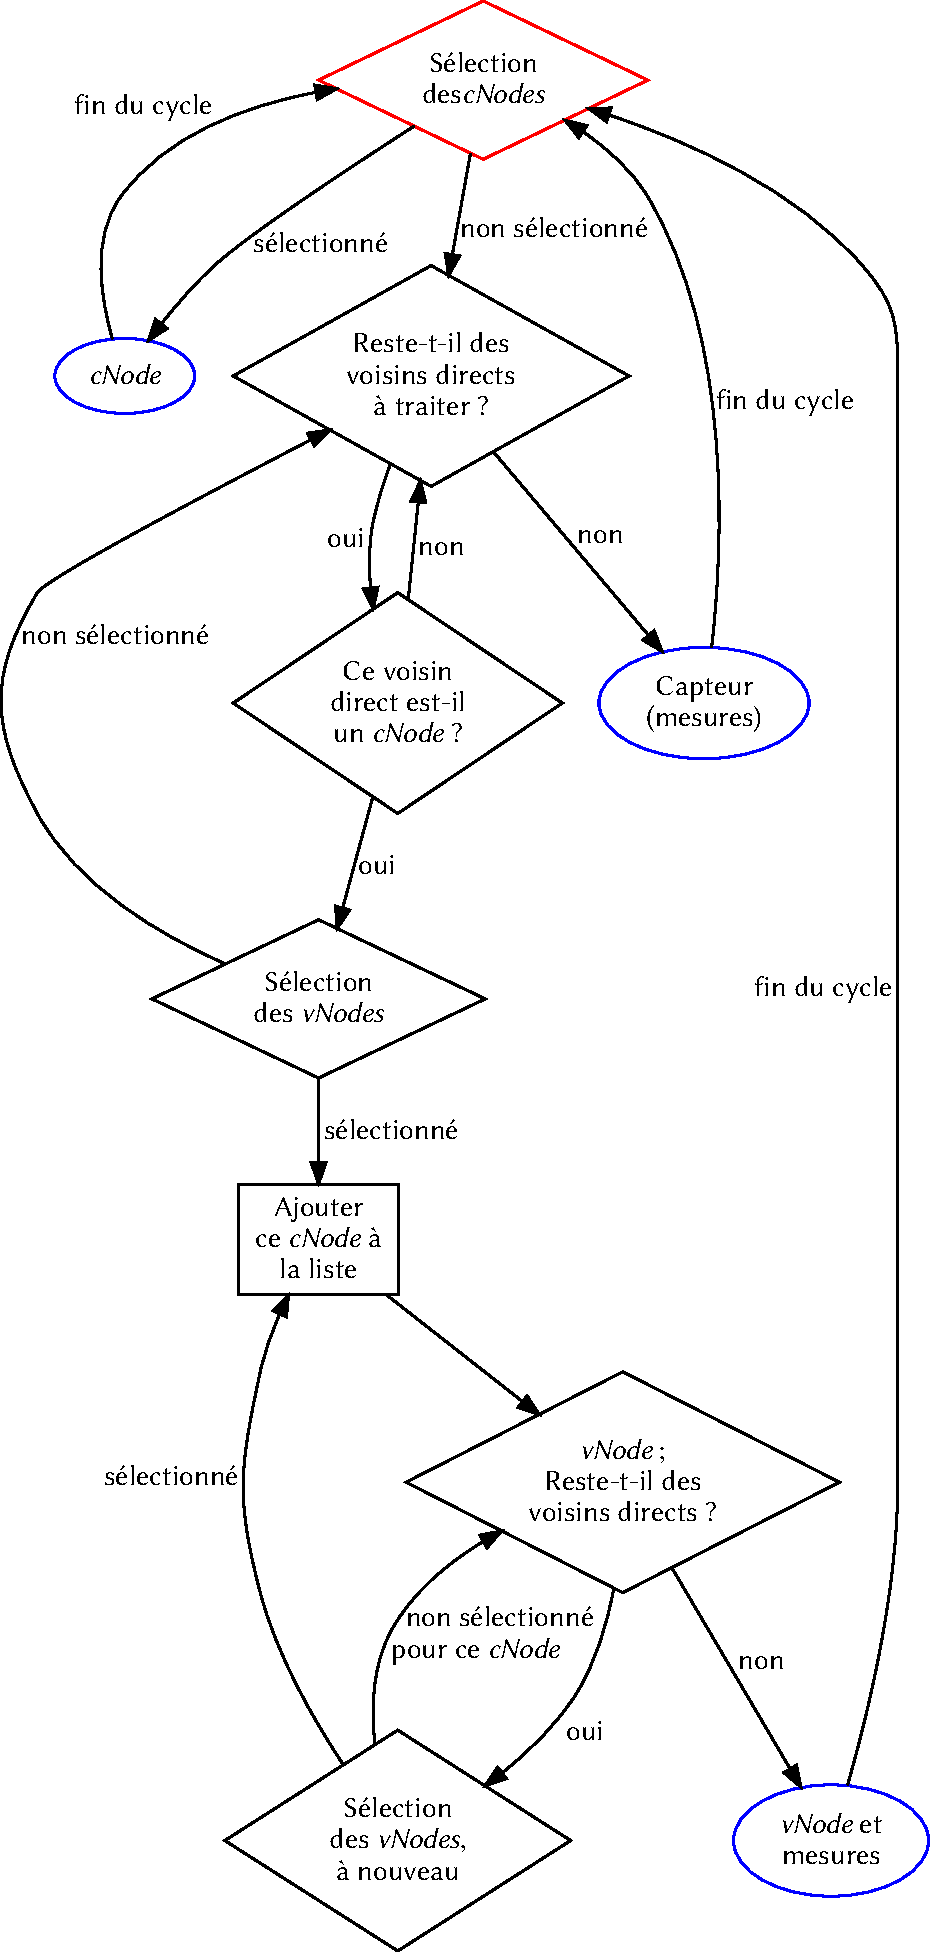
\includegraphics[height=\figuretotextheight]{\chapterfig/state_graph_vert.pdf}%
    \caption{Machine à états des capteurs (non-\cn)}\label{se:fig:states}%
\end{figure}

    \subsection{Couverture du cluster en cas d'activité hétérogène}

Le passage d'un algorithme pseudo-aléatoire à un processus de sélection déterministe n'a pas pour seul inconvénient d'introduire une faille que des capteurs compromis pourraient tenter d'exploiter.
Il soulève un second problème, indépendant du comportement des nœuds, qui pourrait gêner la détection de capteurs compromis.
S'il advient qu'une certaine zone géographique du cluster produit un trafic plus important que le reste des nœuds, alors l'énergie des capteurs de cette zone diminuera plus rapidement.
Il s'ensuit mécaniquement que les \cns ne seront pas ou peu sélectionnés parmi les capteurs de cette zone.
Il y a même de forte chances que les $n$ \cns désirés soient sélectionnés en dehors de la zone en question, et que certains capteurs ne soient pas surveillés du tout tant que le trafic de la zone d'activité ne diminue pas ---~potentiellement pour tous les cycles.
La figure \figref{se:fig:cover} illustre ce problème.
\begin{figure}[ht]
    \centering
    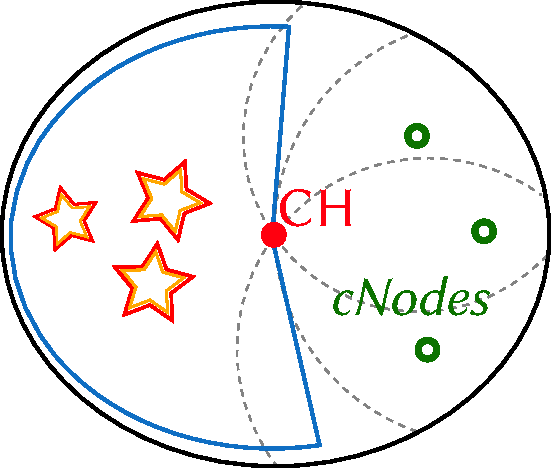
\includegraphics[width=.8\linewidth]{\chapterfig/cover.pdf}
    \caption{Schéma d'explication: les \cns sont sélectionnés au sein de la zone où l'activité est la plus faible (donc ou les nœuds ont conservé le plus d'énergie), et leur surveillance ne couvre pas les capteurs situés dans la partie opposée du cluster.}\label{se:fig:cover}
\end{figure}

Pour assurer une couverture complète du réseau, il est nécessaire de s'assurer que chaque capteur est surveillé par au moins un \cn.
Aussi l'algorithme de sélection présenté plus haut doit-il être modifié, pour devenir:
\begin{enumerate}
    \item Au cours d'une première phase, chaque nœud évalue la valeur de son énergie résiduelle et la transmet au \ch;
    \item Le \ch écoute toutes les valeurs. Les autres nœuds enregistrent également les valeurs de leurs voisins;
    \item Tous les nœuds envoient au \CH la liste de leurs voisins directs (\textit{1-hop})\,\footnote{Nous supposons ici que les capteurs ne trichent pas durant cette étape. Ils pourraient en effet annoncer des voisins «virtuels» supplémentaires, pour faire croire qu'ils seront à portée d'un \cn, et ainsi éviter d'être détecté si ce n'est pas le cas. Le \chapref{ea} présente des mécanismes de protection permettant de détecter ce type d'attaques.};
    \item Le \CH sélectionne les $n$ \cns parmi les nœuds ayant le plus d'énergie résiduelle, de telle façon que ces $n$ nœuds couvrent tous les autres nœuds en terme de portée\,\footnote{Les détails de l'algorithme utilisé pour cette phase ne sont pas précisés dans cette étude.};
    \item Au besoin (si $n$ est trop bas), le \CH sélectionne des \cns supplémentaires de façon à ce qu'ils couvrent l'intégralité du cluster;
    \item Le \CH envoie un message aux nœuds sélectionnés pour leur notifier leur rôle de \cn.
\end{enumerate}

Il est intéressant de noter que certains algorithmes de clusterisation (\heed~\cite{YF04} par exemple) utilisent d'autres mécanismes de sélection basés sur l'énergie résiduelle des nœuds ---~pour choisir des \chs, mais qui pourraient être transposer à la sélection des \cns.
Nous ne souhaitons pas utiliser dans ce chapitre de telles solutions qui n'utilisent l'énergie que comme l'un des paramètres pris en compte, et reposent donc sur la confiance vis à vis des nœuds qui calculent leur score propre.
Au contraire, nous préférons obtenir l'énergie annoncée par les nœuds pour la comparer au modèle théorique, et permettre ainsi aux \vns de veiller à la sécurité du processus.

    \subsection{Observations}

\paragraph{Mécanisme de détection}
La détection des attaques par \dds est inchangée par rapport au chapitre précédent.
Les \cns appliquent un ensemble de règles sur le trafic collecté dans le cluster: lorsqu'un capteur enfreint une règle un certain nombre de fois, par exemple lorsque le débit des paquets qu'il envoie excède un seuil prédéterminé, il est considéré comme malveillant (voir le paragraphe à ce sujet au \chapref{ea}, \ssref{ea:par:rules}).

\paragraph{Alourdissement du modèle}
La solution introduite de par le recours aux \vns consiste littéralement à choisir des nœuds chargés de surveiller les surveillants: le concept de surveillance devient récursif.
Le processus de sélection lui-même est alourdi par les messages des nœuds à destination de leur \ch, annonçant leur énergie résiduelle et la liste de leurs voisins.
Il est évident que la complexité de l'algorithme de sélection, et par suite logique celle de l'implémentation du système, s'en retrouvent rehaussées par rapport au mécanisme de sélection pseudo-aléatoire des \cns.

\paragraph{Allègement possible}
Les \vns sont utilisés pour empêcher les nœuds compromis de conserver un rôle de \cn sur plusieurs cycles sans être détectés.
Lors du premier cycle où un nœud donné occupe le rôle de \cn, il n'y a donc guère d'intérêt à le surveiller: il est statistiquement plus probable qu'il s'agisse d'un nœud légitime plutôt que compromis, et il a de bonnes chances d'abandonner le rôle au cycle suivant.
Le rôle de \vn pour un \cn donné peut donc attendre, pour être assigné, le deuxième cycle consécutif pendant lequel le \cn occupe son rôle.

\paragraph{Sécurité du réseau}
Il est intéressant de se pencher sur un autre point: l'usage des \cns combinés aux \vns n'apporte pas de garantie totale sur la sécurité du réseau.
Le système repose sur plusieurs hypothèses, comme le fait que des nœuds compromis ne collaborent pas ensemble: un capteur compromis sélectionné comme \cn pourrait annoncer au \ch, par exemple, qu'il peut entendre et surveiller une portion plus large du cluster que ce qu'il en est réellement, dans le but de faire croire au \CH que tout le cluster est surveillé~--- alors qu'en réalité ce ne sera pas le cas.
Si le \CH ne désigne aucun autre \cn pour surveiller ces zones, d'autres nœuds compromis pourraient y porter des attaques sans risque d'être détectés.
Une seconde hypothèse à prendre en compte établit que le \ch n'est pas et ne peut pas être compromis.
Une troisième condition à l'application du modèle est d'être en mesure de contenir les tentatives d'usurpation d'identité (voir le \chapref{ea}, \ssref{ea:ssec:auth}), sans quoi un nœud compromis n'a qu'à simuler une identité différente à chaque tour, possédant une batterie (soit disant) pleinement chargée, pour obtenir systématiquement le rôle convoité.
Mais une nouvelle fois, la sécurité d'un système est avant tout une affaire de compromis: plus on cherche à bloquer d'attaques, plus la complexité augmente.

\paragraph{Outils de modélisation}
Si ce chapitre ne présente aucune modélisation formelle du processus introduit, le système n'en a pas moins fait l'objet d'une modélisation, dans une autre étude~\cite{HMMBA14}, sous forme d'automates temporels, dont des propriétés ont été exprimées à l'aide d'un sous-ensemble de CTL (\textit{Computation Tree Logic}, «logique d'arbre de calcul» en anglais) pour être vérifiées à l'aide de l'outil de \textit{model checking} \textsc{Uppaal}\,\footnote{Il ne s'agit cette fois pas d'un sigle, mais d'un nom composé à partir des deux principaux établissements qui ont contribué à l'élaboration de l'outil: le département d'informatique de l'université d'Uppsala (UPP) en Suède, et le département d'informatique de l'université d'Aalborg (AAL) au Danemark.}~\cite{BDL04, uppaal}.
\nomenclature{CTL}{\textit{Computation Tree Logic}}


% vim: set spelllang=fr foldmethod=marker:
\section{Simulation du processus}\label{se:sec:simul}

    \subsection{Résultats numériques}
Le processus de sélection des \cns selon leur énergie résiduelle a, lui aussi, conduit à la réalisation de plusieurs simulations, afin de le comparer au modèle de sélection pseudo-aléatoire.
Le logiciel \nsiii~\cite{ns3} a été utilisé pour l'occasion.

Plusieurs instances de simulation ont été réalisées, avec l'accent porté sur les valeurs de l'énergie consommée ainsi que sur la répartition de la charge dans le cluster.
Les mécanismes de détection des deux méthodes sont quasiment identiques, et fournissent donc des résultats similaires à ceux obtenus au chapitre précédent en \ssref{sa:ssec:detec} (sur la méthode avec renouvellement périodique) pour ce qui est du taux de détection des nœuds compromis.
Les paramètres utilisés lors des simulations sont présentés en \tabref{se:table:parameters}.

\begin{table}[!ht]
    \centering
    \caption{Paramètres de simulation}
    \medskip
    \begin{tabular}{l l}
        \toprule
        \textsc{Paramètre}                 & \textsc{Valeur}\\
        \midrule
        Nombre de nœuds                    & 30 (plus 1~\CH)\\
        Nombre de \cns                     & 4\\
        Probabilité de sélection d'un \vns & 33~\%\\
        Période de renouvellement des \cns & 1~minute\\
        Durée totale de simulation         & 30~minutes\\
        Forme du cluster                   & carré\\
        Taille du cluster                  & 2$\times$50~mètres de diagonale\\
        Portée de transmission             & 50~mètres\\
        Position des nœuds                 & \CH: au centre; autres: aléatoire\\
        Mobilité des nœuds                 & nulle\\
        Débit d'émission des nœuds normaux & 1024~octets toutes les 3~secondes\\
        Requêtes des \vns (par \cn cible)  & 1024~octets toutes les 5~secondes\\
        \bottomrule
    \end{tabular}\label{se:table:parameters}
\end{table}

Ces simulations ont permis d'obtenir l'énergie résiduelle de chaque capteur à intervalles réguliers (une fois par minute).
À partir de ces données, nous avons pu retracer les courbes d'évolution de la moyenne et de l'écart-type de la distribution de l'énergie résiduelle entre les nœuds.
L'énergie résiduelle du \ch a été volontairement ignorée.
\begin{figure}[!b]
    \centering
    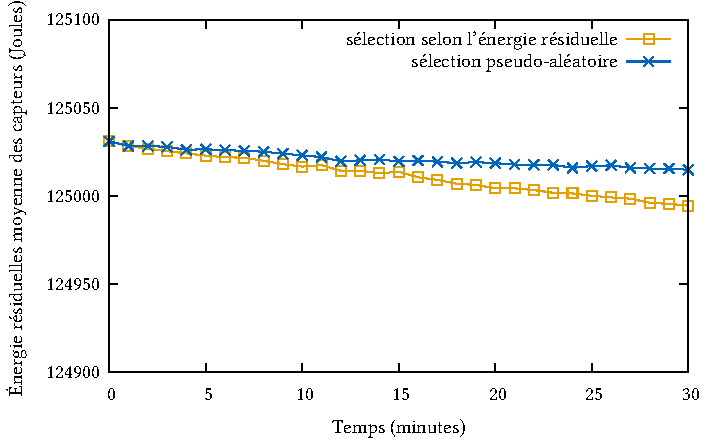
\includegraphics[width=.96\linewidth]{\chapterfig/plot_se_mean.pdf}
    \caption[Valeur moyenne de l'énergie des nœuds en fonction du temps]{Valeur moyenne de l'énergie des nœuds (à l'exception du \ch) en fonction du temps}\label{se:fig:mean}
\end{figure}
La valeur moyenne est présentée sur la \figref{se:fig:mean}.
L'augmentation des valeurs à $t=11$~minutes ainsi qu'à $t=15$~minutes sur la courbe de la sélection par l'énergie provient de l'effet de récupération des batteries.
Ces résultats sont conformes aux attentes: le processus de sélection par l'énergie consomme davantage d'énergie dans le réseau, ce que l'on peut imputer au rôle supplémentaire de \vn mis en place.
Étant donné que les \vns vont avoir à sortir périodiquement de leur état de veille pour envoyer une requête au \cn surveillé, écouter la réponse, et calculer une consommation théorique, le besoin en ressources énergétiques se retrouve logiquement affecté par rapport au processus de sélection pseudo-aléatoire.

Le volume de données de contrôle pour les deux méthodes proposées apparait sur la \figref{se:fig:overhead}.
Ici encore, l'usage des \vns entraine une augmentation des ressources consommées; il faut également tenir compte des messages (moins nombreux) envoyés par chaque capteur au moment du renouvellement de la sélection.
\begin{figure}[!ht]
    \centering
    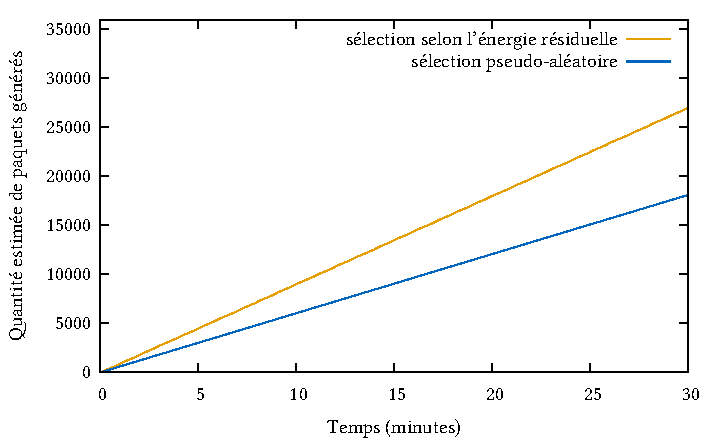
\includegraphics[width=.96\linewidth]{\chapterfig/plot_se_overhead.pdf}
    \caption{Estimation du nombre total de paquets générés au cours de la simulation au cours du temps}\label{se:fig:overhead}
\end{figure}

L'écart-type de la distribution en énergie résiduelle des nœuds est présenté sur la \figref{se:fig:stddev}.
Durant les premières minutes de la simulation, la sélection par l'énergie crée une dispersion plus affirmée de la charge en énergie du réseau, à cause des \vns (il y a davantage de capteurs qui endossent des rôles consommant plus d'énergie).
Mais après les sept premières minutes environ, l'écart-type pour le processus de sélection par l'énergie devient et demeure inférieur à celui associé à la méthode pseudo-aléatoire.
Cela traduit la meilleure répartition de la charge énergétique dans le cluster, ce qui était l'objectif initial de la solution proposée dans ce chapitre.
La différence entre les écart-types des deux méthodes est malgré tout peu élevée: cela tient entre autres aux modèles implémentés pour les simulations.
Comme nous disposons d'un générateur de nombres pseudo-aléatoires efficace, à partir d'un certain nombre de renouvellements de la sélection, tous les capteurs vont endosser le rôle de \cn à peu près le même nombre de fois si la sélection se fait de façon pseudo-aléatoire.
Et comme les capteurs ont également des activités de mesure identique, cette méthode (pseudo-aléatoire) fournit, dans notre cas, une excellente répartition de la charge dans le cluster.
Dans une situation où les capteurs auraient des niveaux d'activité différents ---~si par exemple un évènement à détecter se produit beaucoup plus souvent dans une certaine région géographique du cluster~--- alors la consommation, avec cette méthode, ne serait plus nécessairement équilibrée entre tous les nœuds du cluster.
Tandis que la sélection des \cns par l'énergie résiduelle permettrait de rétablir cet équilibre.
\begin{figure}[!ht]
    \centering
    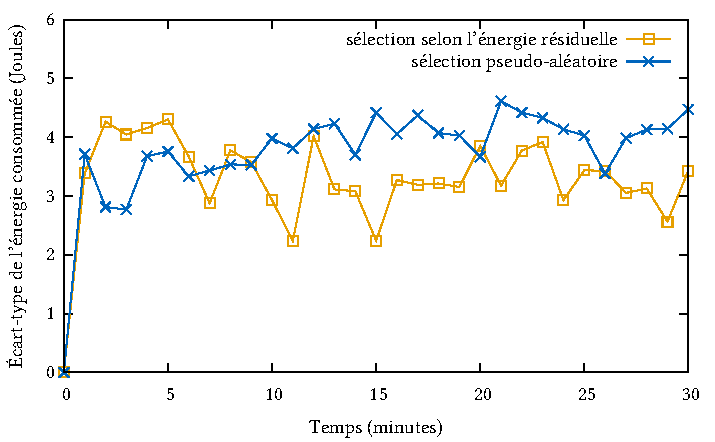
\includegraphics[width=.96\linewidth]{\chapterfig/plot_se_stddev.pdf}
    \caption[Écart-type pour l'énergie résiduelle des nœuds au cours du temps]{Écart-type pour l'énergie résiduelle des nœuds (à l'exception du \ch) au cours du temps}\label{se:fig:stddev}
\end{figure}

    \subsection{Pousser plus loin l'amélioration}

Par rapport au processus d'auto-désignation pseudo-aléatoire introduit dans le chapitre précédent, le second mécanisme proposé prend en compte l'énergie résiduelle de chaque nœud au moment de renouveler les \cns, ce qui assure une meilleure répartition de la consommation en énergie dans le cluster.
Mais si elle est mieux répartie, l'énergie consommée l'est aussi en plus grande quantité, principalement à cause de l'usage nouveau des \vns.
Les requêtes et les réponses aux \cns consomment de l'énergie, et viennent alourdir l'implémentation de la solution: il y a trois rôles différents assignés dans le cluster (sans compter le \ch), et deux d'entre eux nécessitent une étape spécifique pour leur attribution.

Il serait commode de pouvoir se passer des \vns, mais sans faire de concessions sur la sécurité.
L'idéal serait de pouvoir réutiliser les observations des \cns antérieurs pour mettre en place un mécanisme de sélection qui tienne compte de l'énergie résiduelle, voire même d'un ensemble de paramètres permettant de choisir les meilleurs candidats.
Ce jeu de paramètres, s'il inclue un score de confiance, peut même venir renforcer la sécurité du dispositif.
C'est sur cet axe que s'appuient les améliorations proposées dans le prochain chapitre.


\section{Conclusion}

\cns are used in clustered \wsns to monitor traffic of the nodes and to detect \dos attacks (\eg flooding, black hole attacks).
In this paper, we have proposed a new method to dynamically elect those \cns, based on their residual energy.
The aim of the proposed selection algorithm is to provide a better load balancing in the cluster.

We have addressed several issues related with the use of a deterministic selection.
Compromised nodes trying to systematically take over the \cn role are forced to abandon it for later cycle, or get detected, by \vns.
The \vn role is a new role we introduced to survey the \cns by matching their announced energy consumption with a theoretical model.
The issue of areas of the cluster uncovered by \cns, depending of the activity in the cluster, is addressed by enforcing covering of the whole cluster: the \ch is to designate additional \cns if needed.
Working with clusters ensures a good scalability of the solution.
It is also flexible, as \cns can endorse various trust-based model, and monitoring rules can be set to fight against several types of \dos attacks.
And the use of \vns is resilient to a small percentage of compromised \vns (depending on parameters set by user).

The results we have obtained through simulations show that even though using our simulation causes a higher global consumption of energy in the cluster, it provides a better load repartition between sensors.

Future works include improvements of our solution by adding monitoring of the \ch, as well as modeling a cluster with areas of different activity levels.
Also we would especially like to study the impact of the percentage of designated \vns on global energy consumption.


%===============================================================================
%===============================================================================
%   BIBLIOGRAPHIE
%===================
\bibliography{biblio,onrequest}
\bibliographystyle{IEEEtran} %unsrt %plain %alpha
%===============================================================================
\end{document}
